\chapter{Fotometria}\label{ch:fotometria}
\epigraph{La fotometria}{ciao}
\noindent\yinitpar{\color{purple}L}\textsc{a fotometria} è lo studio della radiazione elettromagnetica come detto prima bla bla bla. \lipsum[1]
\section{Intensità, flusso, magnitudini}
    Introduciamo le grandezze più importanti della fotometria. Come sappiamo, la radiazione elettromagnetica trasporta un'energia; supponiamo di avere quindi della radiazione che attraversa una superficie $\dd A$ il cui vettore normale forma un angolo $\vartheta$ con la direzione di propagazione. Essa, lasciando la superficie ``alle sue spalle'', si manterrà all'interno di un angolo solido $\dd\Omega$ che stacca dalla normale alla superficie lo stesso angolo $\dd\vartheta$. In generale le radiazione può contenere qualisai lunghezza d'onda: consideriamo inizialmente la radiazione nelle frequenze comprese nell'intervallo  $\bqty{\nu,\nu + \dd\nu}$. L'energia infinitesima che la radiazione trasporta nella regione $\dd\Omega$ sarà quindi $\dd E_\nu \propto \dd t \dd\nu \cos\vartheta\dd A$. Chiamiamo \emph{intensità specifica} la costante di proporzionalità, $I_\nu$, e scriviamo:
    \begin{equation}
        \label{intensità-specifica-freq}
        \dd[4] E_\nu = I_{\nu} \dd{\nu} \dd{t} \cos{\vartheta} \dd{A} \dd{\Omega}
        \myperiod
    \end{equation}
    In modo del tutto analogo possiamo fare lo stesso ragionamento decomponendo lo spettro in lunghezza d'onda anziché in frequenza e avremo:
    \begin{equation}
        \label{intensità-specifica-lambda}
        \dd[4] E_\lambda = I_\lambda \,\dd\lambda\,\dd t\cos\vartheta\,\dd A \,\dd\Omega
        \myperiod
    \end{equation}
    Integrando su tutte le frequenze otteniamo l'\emph{intensità totale} denotata dalla lettera $I$ e data da
    \begin{equation*}
        \label{intensità-totale}
        \dd[3] E = \int_{0}^{\infty}I_\nu \,\dd\nu\,\dd t\cos\vartheta\,\dd A \,\dd\Omega = I \,\dd t\cos\vartheta\,\dd A \,\dd\Omega
        \myperiod
    \end{equation*}
    Invertendo queste relazioni si trova subito:
    \begin{align}
        I_\nu &= \frac{1}{\cos\vartheta}\frac{\dd[4] E_\nu}{\dd{\nu} \dd{t} \dd{A} \dd{\Omega}} \mycomma \\
        I_\lambda &= \frac{1}{\cos\vartheta}\frac{\dd[4] E_\lambda}{\dd{\lambda} \dd{t} \dd{A} \dd{\Omega}}
        \mycomma \\
        I &= \frac{1}{\cos\vartheta}\frac{\dd[3] E}{\dd t \dd{A} \dd{\Omega}}
        = \int_{0}^{\infty}I_\nu \,\dd\nu
        = \int_{0}^{\infty}I_\lambda \,\dd\lambda
        \myperiod
    \end{align}
    Un'altra grandezza utile nell'Astrofisica è il \emph{flusso di energia}, detto atrimenti \emph{flusso} o \emph{luminosità} che coincide con la potenza. Risulta utile inoltre introdurre la \emph{densità di flusso}---che, purtroppo, viene spesso detta \emph{flusso} creando non poca confusione---ovvero la grandezza che integrata su una superficie restituisce il flusso. In questo modo si ha:
    \begin{align}
        \label{eq:lumin-1}
        L &= \dv{E}{t} = \oint\nolimits_{S} F\dd{S} \mycomma \\
        \label{eq:lumin-2}
        L &= 4\pi r^2 F \quad \implies \quad F = \frac{L}{4\pi r^2}
        \mycomma
    \end{align}
    dove l'ultima uguaglianza è ottenuta integrando su una superficie sferica $S$ di raggio $r$ e supponendo $F$ ivi costante.

    Possiamo dedurre che, se la luminosità è una proprietà intrinseca del corpo che emette radiazione---si pensi alla conservazione della potenza nel vuoto, la densità di flusso allora è una grandezza che decresce con $r^2$. Volendo fare un'analogia con l'elettrostatica, $L$ gioca il ruolo della carica\footnote{A rigore, la carica divisa per $\epsilon_{0}$.} netta di una distribuzione contenuta all'interno di una superficie chiusa ed $F$ quello del campo elettrico da essa generata.

    Se un corpo è esteso e non approssimabile come puntiforme, la luminosità e la densità di flusso saranno funzione delle coordinate di ciascun punto del corpo esteso che le genera. Si definisce \emph{brillanza superficiale} la somma (l'integrale) di tutti i contributi di densità di flusso al variare delle sorgenti elementari.
    \subsection{Magnitudine apparente}
        Un primo tentativo di classificazione delle stelle fu fatto da un astronomo di nome Ipparco nel 129 a.C. Egli divise le stelle in sei classi a seconda di quanto apparissero ``brillanti'' a occhio nudo e chiamò queste classi \emph{magnitudini}. Secondo la sua classificazione le stelle più brillanti andavano collocate nella \emph{prima magnitudine}, seguite da quelle di \emph{seconda magnitudine} \myetc, fino a quelle appena visibili che appartenevano alla \emph{sesta magnitudine}.

        Nel 1956, l'astronomo britannico Norman Pogson formalizzò ed estese questa classificazione matematicamente. Pogson si rese conto che il legame tra la densità di flusso di una stella e la sua appartenenza a una cerca classe di magnitudine di Ipparco era tutt'altro che lineare. Supponendo infatti di avere tre stelle i cui \emph{flussi}\footnote{Qui si fa riferimento alla \emph{densità di flusso}. Per brevità anche in questo testo in alcuni punti si userà l'espressione abbreviata. Per non fare confusione, l'usuale \emph{flusso} verrà chiamato sempre \emph{luminosità}.} siano in rapporto $1:10:100$, la differenza di magnitudine tra la prima e la seconda e tra la seconda e la stessa appare la stessa: se la prima stella è di prima magnitudine e la seconda è di terza magnitudine, la terza apparirà di quinta magnitudine. Pogson in particolare notò che a due stelle i cui i flussi sono in un rapporto di $1:100$ corrisponde una differenza di magnitudine pari a $5$; questo vuol dire che a due classi consecutive di magnitudine deve corrispondere un incremento---o decremento---del flusso un fattore $\sqrt[5]{100} \approx \num{2,512}$. Pogson stabilì quindi che la differenza di magnitudine tra due stelle dovesse essere data dalla relazione
        \begin{equation}
            \label{eq:magnitudine-diff}
            m_{2} - m_{1} = -2.5 \Log{\pqty{\frac{F_{2}}{F_{1}}}}
            \mycomma
        \end{equation}
        dove il \num{-2.5} al posto del \num{-2,512} è intenzionale e $\Log \equiv \log_
        {10}$. Naturalmente la \eqref{eq:magnitudine-diff} non permette di definire univocamente la magnitudine apparente di una stella ma solo di valutare la differenza di magnitudine tra due di esse.\footnote{Un po' come il potenziale di una forza che è definito a meno di una costante ma la d.d.p. è univocamente determinata.} Si usa quindi scegliere una certa stella che abbia un certo flusso $F_{0}$ noto a cui viene imposta una magnitudine $m_{0} = 0$; per convenzione questa scelta ricade sulla stella Vega. In questo modo la \eqref{eq:magnitudine-diff} diventa
        \begin{equation}
            \label{magnitudine-app}
            m = -2.5 \Log{\pqty{\frac{F}{F_{0}}}}
            \myperiod
        \end{equation}
        La magnitudine apparente del Sole, avendo posto Vega a $0$, risulta negativa e pari a \num{-26}. Questo significa che il flusso del sole è circa \num{e10} volte quello di Vega. L'oggetto meno luminoso mai misurato possiede invece una magnitudine apparente di \num{30}. Per rendere un'idea di quanta luce provenga effettivamente da Vega, basti pensare che, in \SI{1}{s}, \SI{1}{cm^2} di superficie è attraversato da circa \num{900} fotoni in un range di lunghezze d'onda di \SI{1}{\angstrom}. Da una lampada invece ne provengono circa \num{e20}.

        È evidente che a magnitudini più basse---o addirittura a valori negativi---corrispondono oggetti più apparentemente luminosi.
    \subsection{Magnitudine assoluta}
        Il fatto che il Sole abbia una magnitudine così ``bassa'' rispetto a tutte le altre stelle non deve indurci a credere che il sole sia effettivamente \num{e10} o più volte più luminoso di esse. Il Sole risulta così fuori scala per via della sua distanza.

        Se teniamo conto del fatto che la magnitudine apparente è definita attraverso il rapporto delle \emph{densità di flusso}, è facile convincersi del fatto che essa non dia alcuna informazione sulla luminosità intrinseca dei corpi celesti considerati. Infatti il flusso decresce col quadrato della distanza e, se immaginiamo di avere stelle identiche a distanze diverse, queste appariranno con magnitudini diverse nonostante la luminosità sia la stessa. Al fine di introdurre un modo più sistematico di valutare la luminosità delle stelle, immaginiamo di prendere tutte le stelle dell'Universo e metterle alla stessa distanza dal nostro punto di osservazione. A questo punto la differenza di magnitudine tra due stelle sarà coerente con la differenza delle loro luminosità---e anche del loro flusso, vista la \eqref{eq:lumin-2}: una stella più luminosa avrà un flusso maggiore e una magnitudine ``più negativa'' e, viceversa, a stelle meno luminose corrisponderanno magnitudini più alte.
        
        Se decidiamo di scegliere questa distanza pari a \SI{10}{\parsec}, otteniamo quella che viene detta \emph{magnitudine assoulta}. La magnitudine assoluta si indica con la lettera $M$ e lega la magnitudine apparente di una stella alla sua distanza da noi. Infatti se indichiamo con $F_r$ il flusso di una stella a distanza $r$ e con $F_{10}$ il suo flusso a distanza \SI{10}{pc}, si ha dalla \eqref{eq:lumin-2}
        \begin{equation*}
            \frac{F_r}{F_{10}} = \frac{4 \pi \pqty{\SI{10}{\parsec}}^2}{4 \pi r^2} = \pqty{\frac{\SI{10}{\parsec}}{r}}^2
        \end{equation*}
        che, inserito nella \eqref{eq:magnitudine-diff} dà
        \begin{equation*}
            m - M = -2.5 \Log{\pqty{\frac{\SI{10}{\parsec}}{r}}}^2
            \myperiod
        \end{equation*}
        Portando un $-2$ fuori dal logaritmo si ottiene quello che viene detto \emph{modulo della distanza}:
        \begin{equation}
            \label{eq:modulo-distanza}
            m - M = 5 \Log{\pqty{\frac{r}{\SI{10}{\parsec}}}}
        \end{equation}
    \subsection{Magnitudine fotografica e bolometrica}
        Fin'ora nel parlare di magnitudini abbiamo completamente trascurato un'informazione importante. Il flusso di una stella dovrebbe essere calcolato tenendo conto di tutti i fotoni ricevuti a tutte le lunghezze d'onda, cosa che di certo l'occhio umano non può fare.
        
        Potremmo provare a migliorare la nostra classificazione con l'aiuto di un sensore \ccd, che ha un'efficienza quantica superiore a quella dell'occhio umano e permette di fare anche esposizioni più lunghe migliorando il rapporto segnale--rumore. Il primo a fare un tentativo simile fu l'astronomo G. P. Bond nel XIX Secolo che ebbe l'intuizione di porre una lastra fotografica sul piano focale di un telescopio. Fotografando diversi oggetti notò che quelli più luminosi lasciavano sulla lastra delle ``macchie'' più grandi e questo permetteva di asssegnare loro una magnitudine in modo più sistematico. Una magnitudine definita in questo modo può risultare sufficientemente utile da avere un nome suo, quello di \emph{magnitudine fotografica}.

        Se provassimo a fare la stessa cosa, con una \ccd---ma anche con una lastra fotografica---dopo poche misurazioni inizieremmo a notare delle discrepanze tra le magnitudini fotografiche e quelle \emph{visuali}:\footnote{Dall'osservazione a occhio nudo.} due stelle con magnitudine visuale uguale potrebbero avere magnitudine fotografica differente e viceversa, oppure nella foto potrebbero comparire stelle invisibili a occhio nudo. Questo è dovuto al fatto che l'efficienza quantica dei sensori \ccd\ non solo è in generale più elevata, ma lo è in un intervallo più esteso di quello dell'occhio umano, con un picco leggermente spostato verso il blu rispetto a quello dell'occhio che ricade nel verde.

        Si definisce invece \emph{magnitudine bolometrica} la magnitudine teorica ottenuta integrando segnale su tutte le lunghezze d'onda alla massima efficienza. Si tratta di una idealizzazione impossibile da ottenere con le misure a causa dei limiti pratici dovuti al mezzo interstellare, l'atmosfera, l'inefficienza degli strumenti \myetc.
\section{Sistema \ubvri\ e indice di colore}
    Un primo modo di risalire alla forma dello spettro di una stella è quello di misurare il flusso di fotoni in alcuni range di lunghezze d'onda---in un modo simile a come costruiremmo un istogramma---per poi ``unire i punti'' e capire in prima approssimazione l'andamento dell flusso con la lunghezza d'onda.
    \subsection{Bande spettrali}
        Si potrebbe pensare che una suddivisione più fine\footnote{Più intervalli, più stretti.} degli intervalli sia utile a migliorare la precisione delle misure, ma purtroppo non è esattamente vero. Ricordiamo che in un intervallo di \SI{1}{\angstrom} una stella di magnitudine $m = \num{0}$ ha un flusso di circa $\num{900}$ fotoni al secondo per centimetro quadrato. Il valore corrispondente per una stella di magnitudine $m = \num{5}$ è di \num{9} fotoni! Se ricordiamo che la ricezione dei fotoni è una misura di conteggio, governata quindi dalla statistica di Poisson, a questi \num{9} fotoni corrisponde un'incertezza del $\SI{33}{\percent}$, che rende la misura statisticamente poco significativa.

        Per migliorare la statistica sarebbe necessario aumentare il tempo di esposizione o la superficie del sensore ma questo è reso difficile dai limiti tecnologici e non è facilmente o sistematicamente estendibile a tutte le lunghezze d'onda. Quello che si sceglie di fare è piuttosto estendere l'intervallo di lunghezze d'onda da misurare ``contemporaneamente'' suddividendole in \emph{bande spettrali} più o meno ampie.
    \subsection{Filtri}
        La standardizzazione di questa tecnica è stata introdotta definendo il sistema \emph{sistema \ubvri} per la suddivisione delle varie bande.
        
        Il modo più intuitivo di selezionare questi intervalli è quello di utilizzare dei materiali come il vetro colorato: quando guardiamo attraverso un vetro rosso, quello che succede è che il vetro blocca le lunghezze d'onda fuori da un certo range e lascia passare quelle in prossimità del rosso. Un oggetto con questo comportamento viene detto \emph{filtro} e ad esso viene assegnata un'importante caratteristica che prende il nome di \emph{trasmissività}, definita come la percentuale di fotoni incidenti che vengono trasmessi. In generale è funzione della lunghezza d'onda (o della frequenza).

        È importante tenere conto della trasmissività quando si eseguono delle osservazioni. Ad esempio se una sorgente emette \num{100} fotoni a una data lunghezza d'onda e questi attraversano un filtro con una trasmissività del \SI{60}{\percent} per poi incidere su un sensore con una efficienza quantica del \SI{50}{\percent}, il sensore rivelerà \num{30} fotoni, meno della metà.

        Il criterio di suddivisione delle bande spettrrali fu affinato nel 1935 da H. L. Johnson che introdusse i primi tre filtri standard indicati dalle lettere U, B e V. Queste stanno per:
        \begin{enumerate}
            \item[\textbf{U:}] Ultravioletto. Il valor medio delle lunghezze d'onda che questo filtro lascia passare è pari a \SI{3650}{\angstrom} (UV).
            \item[\textbf{B:}] Blu. Il corrispettivo valor medio è di \SI{4440}{\angstrom} (violetto--blu).
            \item[\textbf{V:}] Visibile. La sua banda spettrale si colloca verso il centro dello spettro visibile con un valor medio di \SI{5500}{\angstrom} (verde).
        \end{enumerate}
        Questi primi tre filtri sono molto spostati verso il blu perché le lastre fotografiche dell'epoca erano più sensibili a quegli intervalli di lunghezze d'onda. Negli anni successivi si sono introdotti filtri nella direzione dell'infrarosso:
        \begin{enumerate}
            \item[\textbf{R:}] Rosso, con una lunghezza d'onda media di \SI{6400}{\angstrom} (arancione--rosso).
            \item[\textbf{I:}] Infrarosso, con una lunghezza d'onda media di \SI{7900}{\angstrom} (vicino infrarosso).
        \end{enumerate}
        È evidente che il nome del sistema, \emph{\ubvri}, discende proprio da questi cinque filtri.
    \subsection{Indice di colore}
\section{Diagramma di Hertzsprung--Russel}
\section{Estinzione e profondità ottica}
    Quanto detto fin'ora è tecnicamente vero solo se supponiamo di metterci in un contesto ideale dove tra il rivelatore e la stella c'è il vuoto perfetto, cosa naturalemte non vera. La radiazione che parte da una stella viaggia per distanze molto lunghe prima di arrivare a terra e lo spazio tra sorgente e rivelatore è tutt'altro che vuoto. I due principali ostacoli sono l'atmosfera terrestre---per le misure fatte da terra---e il mezzo interstellare, ovvero l'insieme di gas e polveri che permeano in modo non uniforme lo spazio tra i corpi celesti.

    Come si può intuire, i fenomeni che impediscono a tutta la radiazione di giungere al suolo sono vari. Tra i principali ci sono:
    \begin{enumerate}[label=\ding{70}]
        \item diffusione Thomson;
        \item diffusione Compton;
        \item assorbimento e riemissione a lunghezze d'onda diverse da quelle osservate.
    \end{enumerate}
    Il tipo di interazione radiazione--materia dipende dal rapporto tra la lunghezza d'onda $\lambda$ del fotone e la dimensione $d$ delle particelle che costituiscono il materiale:
    \begin{enumerate}[label=\ding{70}]
        \item se $\lambda \ll d$ prevale lo scattering Compton;
        \item se $\lambda \sim d$ prevale lo scattering Thomson;
        \item se $\lambda \gg d$ prevale la trasmissione indisturbata del fotone. 
    \end{enumerate}
    
    Cerchiamo di capire quantitativamente come questi fenomeni alterino la radiazione partendo dal caso in atmosfera.
    \subsection{Estinzione atmosferica}
        L'atmosfera, per quanto sia sottile rispetto alle distanze interstellari, costituisce un ostacolo non indifferente alla propagazione della luce se consideriamo che circa la metà dei fotoni incidenti viene riflessa. Tuttavia l'interazione dipende evidentemente dalla lunghezza d'onda: quando guardiamo il sole al tramonto esso risulterà più rosso e possiamo dunque dedurre che la luce blu interagisce più facilmente con l'atmosfera rispetto a quella rosso--arancione.\footnote{È proprio per questo che il cielo appare azzurro: i fotoni con la lunghezza d'onda del blu sono diffusi e giungono ai nostri occhi da tutte le direzioni, mentre quelli arancioni--rossi proeguono in modo più coerente e fanno apparire il sole più rosso. Questo effetto è particolarmente accentuato al tramonto, dovendo la luce attraversare una porzione più spessa di atmosfera.}

        Cerchiamo adesso di scrivere una relazione che espliciti come l'intensità specifica si trasformi in funzione delle proprietà del materiale che attraversa. Considerato un volumetto di area unitaria e spessore $\dd{x}$; la radiazione di frequenza $\nu$ che incide perpendicolarmente avrà intensità specifica $I_\nu$ e quella che lascia il volumetto sarà, approssimando al primo ordine, $I_\nu + \dd{I_\nu}$.
        \begin{figure}[h]
            \centering
            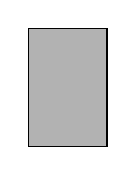
\begin{tikzpicture}
    %\pgfmathsetmacro{\cubex}{1}
    %\pgfmathsetmacro{\cubey}{2}
    %\pgfmathsetmacro{\cubez}{2}
    %\draw (0,0,0) -- (\cubex,0,0);
    %\draw (0,0,0) -- (0,\cubey,0);
    %\draw (0,\cubey,0) -- (\cubex,\cubey,0);
    %\draw (\cubex,0,0) -- (\cubex,\cubey,0);
    %\draw [dashed] (0,0,-\cubez) -- (\cubex,0,-\cubez);
    %\draw [dashed] (0,0,-\cubez) -- (0,\cubey,-\cubez);
    %\draw (0,\cubey,-\cubez) -- (\cubex,\cubey,-\cubez);
    %\draw (\cubex,0,-\cubez) -- (\cubex,\cubey,-\cubez);
    %\draw [dashed] (0,0,0) -- (0,0,-\cubez);
    %\draw (0,\cubey,0) -- (0,\cubey,-\cubez);
    %\draw (\cubex,\cubey,0) -- (\cubex,\cubey,-\cubez);
    %\draw (\cubex,0,0) -- (\cubex,0,-\cubez);
    \pgfmathsetmacro{\cubex}{1}
    \pgfmathsetmacro{\cubey}{1.5}
    \pgfmathsetmacro{\cubez}{1.5}
    \draw[fill=gray!60!] (2.5,0.75,0) -- ++(-\cubex,0,0) -- ++(0,-\cubey,0) -- ++(\cubex,0,0) -- cycle;
    %\draw[fill=gray!80!] (2.5,0.75,0) -- ++(0,0,-\cubez) -- ++(0,-\cubey,0) -- ++(0,0,\cubez) -- cycle;
    %\draw[fill=gray!50!] (2.5,0.75,0) -- ++(-\cubex,0,0) -- ++(0,0,-\cubez) -- ++(\cubex,0,0) -- cycle;
    %\draw[blue!60!cyan!90!, -{Triangle[width = 14pt, length = 8pt]}, line width = 6pt] (2.7, 0.) -- (3.7, 0);
    %\draw[blue, -{Triangle[width = 14pt, length = 8pt]}, line width = 6pt] (0.0, 0.0) -- (1, 0.0);
    %\node at (-0.3,0) {$I_{\nu}$};
    %\node at (4.5,0) {$I_{\nu} + dI_{\nu}$};
    %\draw (1,-0.8) -- (1,-0.9) -- (2.5,-0.9) -- (2.5,-0.8);
    %\node at (1.75,-1.1) {$dx$};
    %\node at (2,0) {$\kappa_{\nu}$};
\end{tikzpicture}
            \caption{Cubetto}
        \end{figure}

        Sperimentalmente si osserva che il $\dd{I_\nu}$ è proporzionale sia all'intensità $I_\nu$ incidente che allo spessore $\dd{x}$ del materiale attraversato: se si raddoppia l'intensità verranno ``persi'' il doppio dei fotoni e lo stesso avviene se si raddoppia lo spessore del materiale attraversato. Naturalmente questa quantità deve dipendere anche dalle proprietà intrinseche del materiale come la densità o la sua composizione molecolare quindi introduciamo il coefficiente di proporzionalità $\kappa_\nu$ che esprime questa dipendenza insieme a quella dalla lunghezza d'onda. Si avrà quindi:
        \begin{equation}
            \label{eq:estinzione-atmosferica-1}
            \dd{I_\nu} = - \kappa_\nu I_\nu \dd{x}
            \myperiod
        \end{equation}
        In alcuni casi può essere utile esplicitare la dipendenza dalla densità $\rho$ ``estraendola'' da $\kappa_\nu$ e scrivendo quindi $\kappa_\nu \to \kappa_\nu\rho$; il coefficiente $\kappa_\nu$ definito esplicitando $\rho$ viene detto coefficiente \emph{di assorbimento} o \emph{di estinzione}.

        Dal momento che in generale in Astrofisica non è possibile sondare tutti i punti del percorso seguito dalla radiazione, la dipendenza da $x$ nella \eqref{eq:estinzione-atmosferica-1} è relativamente inutile. All'estinzione della radiazione che giunge ai nostri strumenti infatti contribuisce la totalità del materiale attraversato e a noi tocca lavorare con questa radiazione ``a conti fatti''. Risulta quindi utile introdurre la \emph{profondità ottica} $\tau_\nu$ ottenuta integrando $\kappa_\nu\rho$, funzioni di $x$, lungo tutto lo spessore di materiale attraversato $L$:
        \begin{equation}
            \label{eq:spessore-ottico}
            \tau_\nu = \int_{0}^{L} \kappa_\nu\pqty{x} \rho\pqty{x} \dd{x}
            \mycomma
        \end{equation}
        essendo $x=0$ l'ascissa---eventualmente curvilinea---del punto di partenza e $x=L$ quella del punto arrivo.

        Fatte queste considerazioni, la \eqref{eq:estinzione-atmosferica-1} si scrive
        \begin{equation}
            \label{eq:estinzione-atmosferica-2}
            \dd{I_\nu} = -I_\nu \dd{\tau_\nu}
            \mycomma
        \end{equation}
        che può essere facilmente integrata ponendo in particolare $I_\nu\pqty{0} = I_{\nu}^{\text{0}}$:
        \begin{equation}
            I_\nu = I_{\nu}^{\text{0}} e^{-\tau_\nu}
            \mycomma
        \end{equation}
        dove la dipendenza da $x$ può essere esplicitata scrivendo
        \begin{equation*}
            I_{\nu}\pqty{x} = I_{\nu}^{\text{0}} \exp[-\int_{0}^{x} \kappa_\nu\pqty{x'} \rho\pqty{x'} \dd{x'}]
            \myperiod
        \end{equation*}
        Osserviamo quindi che gli oggetti con una profondità ottica $\tau_\nu$ molto piccola sono sostanzialmente trasparenti alla luce di frequenza $\nu$; viceversa gli oggetti con una profondità ottica elevata appaiono più opachi.
        
        Quanto detto fin'ora è valido solo nell'ipotesi in cui la radiazione incide perpendicolarmente alla superficie del materiale considerato. Purtroppo, non tutte le stelle si trovano allo zenit quando le osserviamo, quindi è necessario fare delle considerazioni ulteriori.